\documentclass[
a4paper,
oneside,
10pt,
fleqn,
headsepline,
toc=listofnumbered, 
bibliography=totocnumbered]{scrartcl}

% deutsche Trennmuster etc.
\usepackage[T1]{fontenc}
\usepackage[utf8]{inputenc}
\usepackage[english, ngerman]{babel} % \selectlanguage{english} if  needed
\usepackage{lmodern} % use modern latin fonts

% Custom commands
\newcommand{\AUTHOR}{Michael Wieland}
\newcommand{\SECONDAUTHOR}{Fabian Hauser}
\newcommand{\INSTITUTE}{Hochschule für Technik Rapperswil}

% Jede Überschrift 1 auf neuer Seite
\let\stdsection\section
\renewcommand\section{\clearpage\stdsection}

% Multiple Authors
\usepackage{authblk}

% Include external pdf
\usepackage{pdfpages}

% Layout / Seitenränder
\usepackage{geometry}

% Inhaltsverzeichnis
\usepackage{makeidx} 
\makeindex

\usepackage{url}
\usepackage[pdfborder={0 0 0}]{hyperref}
\usepackage[all]{hypcap}
\usepackage{hyperxmp} % for license metadata

% Mathematik
\usepackage{amsmath}
\usepackage{amssymb}
\usepackage{amsfonts}
\usepackage{enumitem}

% Images
\usepackage{graphicx}
\graphicspath{{images/}} % default paths

% Boxes
\usepackage{fancybox}

%Tables
\usepackage{tabu}
\usepackage{booktabs} % toprule, midrule, bottomrule
\usepackage{array} % for matrix tables

% Multi Columns
\usepackage{multicol}

% Header and footer
\usepackage{scrlayer-scrpage}
\setkomafont{pagehead}{\normalfont}
\setkomafont{pagefoot}{\normalfont}
\automark*{section}
\clearpairofpagestyles
\ihead{\headmark}
\ohead{\TITLE}
\cfoot{\pagemark}

% Pseudocode
\usepackage{algorithm}
\usepackage{algorithmic}

% Code Listings
\usepackage{listings}
\usepackage{color}
\usepackage{beramono}

\definecolor{DarkPurple}{rgb}{0.4, 0.1, 0.4}
\definecolor{DarkCyan}{rgb}{0.0, 0.5, 0.4}
\definecolor{LightLime}{rgb}{0.3, 0.5, 0.4}
\definecolor{Blue}{rgb}{0.0, 0.0, 1.0}

\lstdefinestyle{eclipse-style}{
	language=Java,  
	columns=flexible,
	showstringspaces=false,     
	basicstyle=\footnotesize\ttfamily, 
	keywordstyle=\bfseries\color{DarkPurple},
	commentstyle=\color{LightLime},
	stringstyle=\color{Blue}, 
	escapeinside={£}{£}, % latex scope within code      
	morekeywords={length},
	numbers=left,
	numberstyle=\tiny\color{black},
	frame=single,
}
\lstset{style=eclipse-style}


% Theorems \begin{mytheo}{title}{label}
\usepackage{tcolorbox}
\tcbuselibrary{theorems}
\newtcbtheorem[number within=section]{definiton}{Definition}%
{fonttitle=\bfseries}{def}
\newtcbtheorem[number within=section]{remember}{Merke}%
{fonttitle=\bfseries}{rem}
\newtcbtheorem[number within=section]{hint}{Hinweis}%
{fonttitle=\bfseries}{hnt}

% Dokumentinformationen
\newcommand{\SUBJECT}{Report}
\newcommand{\TITLE}{Cloud Infrastructre Lab 6}

\begin{document}
	
% Front page
\title{\TITLE}
\subject{\SUBJECT}
\author{\SECONDAUTHOR}
\author{\AUTHOR}
\affil{\INSTITUTE}
\date{\today}
\maketitle

% Table of contents
\tableofcontents


\section{Modern Data Center Requirements}

Die Ansprüche an ein Data Center haben sich in den letzten zehn Jahren stark gewandelt. In den folgenden Abschnitten werfen wir einen Blick auf die Änderungen der letzten Jahre sowie der neu entstandenen Ansprüche an Data Centers.

% - was ändert sich
% - was ist heutigen DC anders als 20 jahre

\subsection{Network architecture}\label{sec:network-architecture}
\subsubsection{Vor ca. 2008}
Vor ca. 2008 waren Data Center üblicherweise in ''Silos'' aufgeteilt: Jede Abteilung und Applikation hatte meist ein eigenes ''Rack'' mit physischen Servern. Damit war die Struktur eher starr und teuer; Skalierung von Ressourcen war nur mit physischem erweitern der Infrastruktur möglich.

\paragraph{Das Netzwerk} war entsprechend aufgebaut; Subnetze wurden statisch Abteilungen und Applikationen zugewiesen. Dies war möglich, da die Infrastruktur keinen kurzfristigen, grossen Anpassungen erlaubte.

\subsubsection{Seit ca. 2008}
Seit ca. 2008 hält die Virtualisierung in das Data Center Einzug. Damit wird die Umgebung nicht mehr in ''Silos'' aufgeteilt, sondern in ressourcen-Pools für Computation, Storage und Netzwerkvirtualisierung. Das verknüpfen dieser Pools wird durch den Betrieb von virtuellen Servern möglich. Die wesentlichen Vorteile dieser Umgebung lassen sich kurz zusammenfassen auf die...
\begin{itemize}
	\item Reduktion der Komplexität
	\item Vereinfachung des Betriebs
	\item Erhöhung der Auslastungseffizienz (Bündelungsgewinn)
	\item Erhöhte Ausfallssicherheit
	\item Einfachere Skalierung der Infrastruktur
	\item Ermöglichung von Automatisierung
\end{itemize}

Seit 2010 bis heute wird neben der Virtualisierung die Automatisierung von möglichst vielen Komponenten vorangetrieben. Damit wird es möglich, mit weniger personellem Aufwand mehr Server zu betreiben und repetitive Aufgaben autonom (oder teilautonom) erledigen zu lassen.

\paragraph{Das Netzwerk} muss dadurch ebenfalls flexibler und einfacher änderbar sein. Dies wird entweder durch eine ''flachere'' Netzwerkstruktur, oder dem Einsatz von Fabrics erreicht. Allerdings ist der klassische Netzwerkstack nicht für solche Strukturen Designed; hier kommen Protokolle wie TRILL und VXLAN sowie die Virtualisierung von Netzwerkkomponenten ins Spiel.

Weitere Änderungen im Bezug auf den Netzwerkverkehr sind: 
\begin{itemize}
	\item Eine deutlich höhere Auslastung des East-West-Verkehrs: Der Verkehr bleibt eher im Data Center, verursacht wird er z.B. durch das Verschieben von VMs\footnote{Virtuelle Maschinen; siehe Lab 5 für alle Details.}. \hfill \\
		 Pre-2008 gab es in erster Linie Netzverkehr zwischen Clients und Servern.
	\item Sogenannte ''Elephant Flows'' dominieren den Verkehr im Netzwerk (Speicher, Verteilte Datenbanken etc.)
	\item Mehr (kleine) Auslastungsspitzen im Netzwerk; dies kann zu Paketverlust führen.
	\item Betrieb von ''map-reduce'' applikationen, welche viel eingehenden TCP-Netzverkehr haben (many-to-one traffic)
\end{itemize}


\subsection{Challanges}

Durch die in Kapitel \ref{sec:network-architecture} genannten Änderungen in der Netzwerkarchitektur ergeben sich einige neue Challenges:
\begin{itemize}
	\item Es muss viel mehr Netzverkehr East-West fliessen können
	\item Aufgrund der neuen Applikationsarchitekturen und Datengrössen gibt es überhaupt mehr Netzwerkverkehr.
	\item IP-Netze müssen sich über mehrere Nodes (physische und virtuelle Server) erstrecken können
	\item Die Netzwerk-Struktur muss schnell und einfach geändert werden können
	\item Es müssen höhere Lastspitzen abgefangen werden können
\end{itemize}

Einige weitere neuartige Requirements sind auch im nächsten Kapitel~\ref{sec:requirements-an-das-netzwerk} aufgelistet.

\subsection{Requirements an das Netzwerk}\label{sec:requirements-an-das-netzwerk}
Es gibt somit einige neue grundlegende Anforderungen an das Netzwerk\footnote{Quelle u.A. Foliensatz \lstinline|09_Changes in the Datacenter Network Design.pdf| von Prof. B. Stettler.}.
\subsubsection{Eigenschaften Forwarding}
\begin{itemize}
	\item Höhere Geschwindigkeiten (z.B. 10Gbps im Access Layer, 40/100Gbps im Core Layer)
	\item Verstärktes Multipath für L3 und evtl. L2 Traffic, um den East-West Durchsatz zu erhöhen. (Kein Port/Link Blocking wie bei STP)
	\item Weniger Netzwerkhops (zur Senkung der Latenzzeiten)
	\item Optimales L3 Forwarding
	\item Trennung von L3 verkehr (L3 Path Isolation)
	\item IPv6
	\item Speicher- und Netzwerk sind mit mindestens 10GE verbunden (iSCSI oder FCoE)
	\item Verlustfreier Netzwerkverkehr (für DCB)
\end{itemize}

\subsubsection{Control \& Management Funktionen}
\begin{itemize}
	\item Enge Verzahnung des Netzwerks mit den virtuellen Servern
	\item L2 ohne STP (und ähnliche Protokolle, aufgrund Port-Blocking)
	\item Effizientes Management
	\item Einfache Provisionierung / Erweiterung des Netzwerks
\end{itemize}


\subsubsection{Skalierbarkeit}
\begin{itemize}
	\item Hohe Anzahl von VLANs
	\item Grosse Tabellengrössen (MAC, ARP, L3, IPMC etc.)
	\item Schnelles Netz (per Design, auch bei grossen Netzvergrösserungen)
\end{itemize}

\subsubsection{Weitere Anforderungen }
\begin{itemize}
	\item Rechtliche Compliance (Datenschutz/Datensicherheit)
	\item Multitenancy (Abtrennung von mehreren Kunden im selben Netz)
\end{itemize}


\section{TRILL}\label{sec:trill}
\subsection{Terminologie}
\begin{description}
	\item[RBrige] Bridge die TRILL unterstützt und verwendent
	\item[Ingress RBRige] \hfill \\
	Bridges die beim Eingang in die TRILL ''Wolke'' stehen. Sie fügen den TRILL Header hinzu
	\item[Egress RBRige] \hfill \\
	Bridges die beim Ausgang der TRILL ''Wolke'' stehen. Sie entfernen den TRILL Header.
	\item[Transit RBridge]  \hfill \\
	Bridges die den TRILL Verkehr nur weiterleiten und dabei nur den Outer Ethernet Header beachten. Sie stehen innerhalb der TRILL ''Wolke''.
\end{description}

\subsection{Funktion} %function / protocol header
Das TRILL Protokoll  (Transparent Interconnection of Lots of Links) implementiert ein Routing auf Layer 2. Das Routing wird mit sogenannten RBridges vollzogen. RBridges routen die verpackten Ethernet Frames mit dem Link-State-Protokoll IS-IS (Intermediate System to Intermediate System). TRILL kann relativ einfach in eine bestehendes Netz eingefügt werden, da Bridges ohne TRILL Funktion, die restlichen RBridges als Wolke und somit als ein grossen Switch wahrnehmen. (Vergleichbar mit MPLS). \\ 

Versendet ein Client A ein Paket an Client B, wird das MAC Frame bei der Ingress RBrige in ein TRILL Paket verpackt. Anschliessend routet IS-IS das Paket zur Egress Bridge welche den TRILL Header wieder entfernt und das ursprüngliche MAC Frame auspackt.  \\

Edge RBridges (Ingress, Egress) lernen die angeschlossen Clients auf die klassische Art und Weise über ARP. Das Wissen, welche MAC Adresse an welcher Edge RBridge angeschlossen ist, wird dann über IS-IS an die weiteren RBridges verteilt. Da Link State Protokolle über die gesammte Netzwerktopologie bescheid wissen, kann IS-IS optimale Pfade für Unicast, sowie Distribution Trees für unbekannte Hosts und Broadcast und Multicast Gruppen berechnen. Die berechneten Bäume bilden einen Pfad zu allen Egress Bridges ab. Durch das Equal Cost Multipath Routing (ECMP) werden alle Pfade mit gleichen Kosten zu einem Ziel parallel genutzt. Dadurch erreicht man eine höhere Bandbreit, als dies unter STP möglich war. IS-IS verwendet für die Berechnung des kürzestens Wegs den Dijkstra-Algorithmus ein. Dieser garantiert loop-freie Pfade. Zudem wird ein Hop Cound im TRILL Header verwendet um Loops zu unterbinden.

\subsection{Protokoll Header}
Ein TRILL Frame ist in drei Schichten aufgeteilt:
\begin{description}
	\item[Outer Ethernet Header] \hfill \\
	Der äussere Ethernet Header wird bei jedem Hop geändert. Dabei bleibt der innere Header konsistenz (inkl. VLAN Tag). Im Outer Header stehen die MAC Adressen der RBridges.
	\item[TRILL Header] \hfill \\
	Das interessanteste im TRILL Header ist die Ingress-RBridge (Source) und Egress-RBrige (Destination). Jede RBridge wird mit einem Nickname (2Byte Hexadezimal) eindeutig identifiziert. (z.B \lstinline[]|0x56ce|) 
	\begin{itemize}
		\item Hop Count: Wird beim passieren jeder RBridge verkleinert und verhindert dass ein Paket zu loopen beginnt. 
		\item Nickname: Der RBridge Nickname ist eine Abkürzung (2Byte) der 6Byte langen IS-IS System ID der Bridge. Sie ist eindeutig innerhalb eines Netzes. 
		\item M Bit (Multidestination): 0 = Unicast, 1 = Distribution Tree
	\end{itemize}
	\item[Inner Ethernet Header] \hfill \\
	Im Inner Ethernet Header stehen MAC-Adressen der beiden Endstation sowie der VLAN Tag.
\end{description}

\begin{figure}[h]
\centering
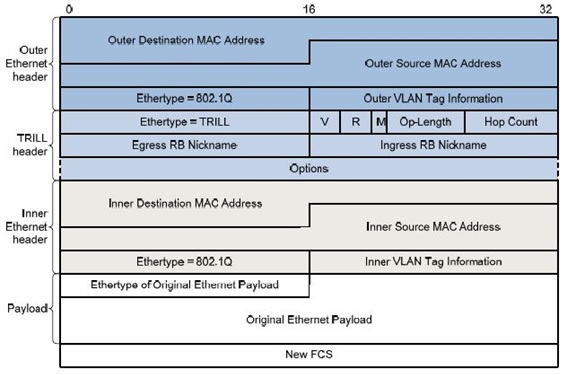
\includegraphics[width=0.6\linewidth]{images/trill_header}
\caption{TRILL Frame}
\label{fig:trillheader}
\end{figure}

\subsection{Ziel von TRILL} %goal of trill
Das Ziel von TRILL ist es auf Layer 2 ein Routing zu betreiben und dabei die Nachteile von STP zu lösen.

\subsection{Warum wurde TRILL entwickelt?} %why was trill developed?
TRILL wurde entwickelt um das Spanning Tree Protocol (STP) zu ersetzen. STP wurde entwickelt um Bridging Loops zu unterbinden. Das Problem bei STP ist, dass es eine relativ grosse Konvergenzzeit hat und Links blockiert, was in Rechenzentren inakzeptabel ist. TRILL wurde entwickelt um genau dieses Problem zu lösen. TRILL verwendet IS-IS (Intermediate System to Intermediate System Protocol) auf Layer 2. IS-IS ist wie OSPF eine Link State Protokoll welches aber im Gegensatz zu OSPF auf L2 operieren kann. Wie alle Link State Protokollen weiss jede RBridge über die gesamte Topologie bescheid. 

\subsection{Wo und wie kann TRILL eingesetzt werden (Use Cases)?} %where and how can trill be used? (use cases)


\subsubsection{High Performance Datacenter}
Bei modernen Datencenter versucht man die Spine-Leaf Architektur umzusetzen. Diese flachen Layer 2 Netze werden oft mit TRILL verwaltet, die STP in der neuen Architektur nicht effizient arbeiten könnten. Aus Spine-Leaf Architektur folgt, dass sehr viele Leaf Switches gibt, die mit jedem Spine Knoten verbunden werden. Die Hohe Anzahl an Verbindungen würde unter STP zu viele blockierten Ports führen.  Da TRILL alle verfügbaren Ports und Pfade nutzt, kann die Payload bei einer maximalen Bandbreite übertragen werden. Damit agiert ein Datacenter in sich extrem performant. 

\subsubsection{VMotion}
Durch den Einsatz von VMotion sind flache Layer 2 Netze nötig, damit die virtuellen Maschienen zwischen mehreren Host Systemen je nach Last verschoben werden müssen. Damit diese Layer 2 Netze performant arbeiten ist ein Protokoll wie TRILL oder SPB nötig. 


\subsection{Ist TRILL kompatibel mit traditionellen Protokollen?} %is trill comparable to a traditional protcol?
%  if yes, what are the differences and which limitiations does TRILL solve?
TRILL ist kompatibel mit VLAN und STP. Der VLAN Tag des Inner Ethernet Header wird bei der Übertragung durch Transit RBridges nicht beachtet. Der VLAN Tag im Outer Ethernet Header wird nur verwendet wenn zwei RBridges über unterschiedliche VLAN's kommunizieren. STP Bridges ohne TRILL Funktionalität erkennen die TRILL ''Wolke'' als einen grossen Switch. TRILL agiert für das restliche 802.1 Netzwerk als eigenständiges System operiert somit oberhalb des klassischen Layer 2. Man kann also sagen, dass TRILL wie MPLS zwischen zwei Layer arbeitet. Bei TRILL wäre dies also Layer 2.5. 


\subsection{Was sind die Vor- und Nachteile von TRILL?}%what are the advantages and disadvantages of TRILL
\subsubsection{Vorteile} \hfill \\
Die Vorteile von TRILL decken sich mit den Kritikpunkten an STP. So gibt es bei TRILL keine blockierten Ports (die ganze Bandbreite kann genutzt werden) und es gibt keine Probleme mit der Konvergationszeit des L2 Netzes. Dadurch kann auf STP verzichtet werden. 
TRILL erlaubt es Virtuelle Maschienen zu verschieben (z.B VMotion) ohne dass man sich Gedanken über die IP Subnetze machen muss.

\subsubsection{Nachteile} \hfill \\
Ein Kritikpunkt an TRILL ist, dass es zu schlechtem Design in den Rechenzentren führe und Alternative Protokolle wie z.B SPB das Problem eleganter lösen. Ebenfalls sind für TRILL spezielle Geräte nötig, was zu erhöhten Initialen Kosten führt.

\subsection{Gibt es andere moderne Technologien, welche TRILL ähnlich sind?}%are there other modern technologies which are similar to TRILL?
%  if yes, what are the differences between them
Der grösste Konkurenz von TRILL ist SPB (Shortest Path Bridging oder IEEE 802.1aq). SPB wurde als Erweiterung von VLAN entwickelt, mit dem gleichen Ziel, um die Konvergenzzeit von STP zu verbessern. SPB verwendet das herkömmliche Header Format, wodurch ohne Hardware Update in ein bestehendes Netzwerk eingefügt werden kann. 


\subsection{Lab Konfiguration}\label{sec:lab-konfiguration}
\begin{figure}[H]
	\centering
	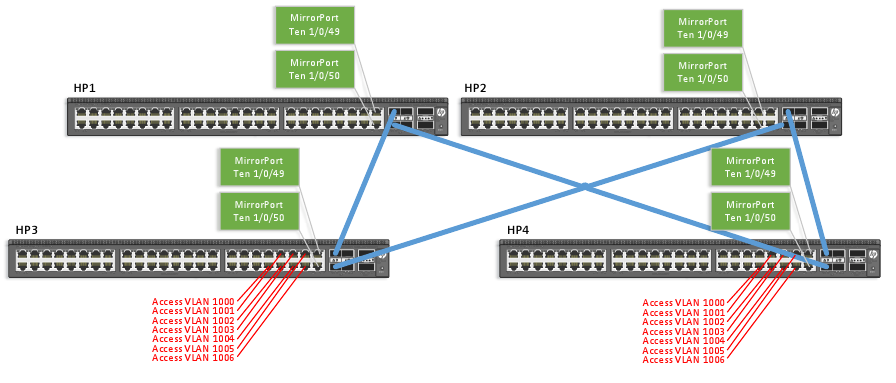
\includegraphics[width=0.7\linewidth]{trill_network_layer2}
	\caption{Lab TRILL Testaufbau}
	\label{fig:trillnetworklayer2}
\end{figure}
\begin{figure}[H]
	\centering
	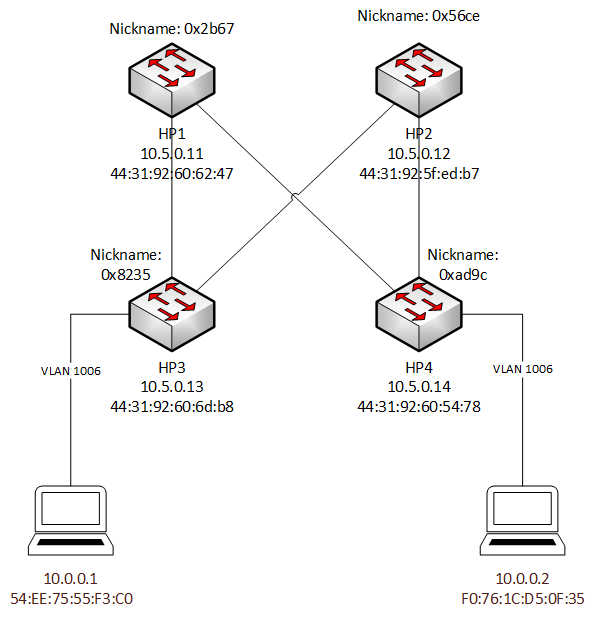
\includegraphics[width=0.7\linewidth]{testaufbau}
	\caption{Lab TRILL Testaufbau}
	\label{fig:testaufbau}
\end{figure}
%TODO: Welcher switch welche funktion.

\begin{table}[H]
	\centering
	\begin{tabu} to \linewidth {l l l l l}
		\toprule
		Switch & Network Entity & TRILL Nick & Nick Prio & Tree Root Prio \\
		\midrule
		HP1 & \lstinline|00.4431.9260.6247.00| & \lstinline|0x2b67| & 192 & 65535 \\
		HP2 & \lstinline|00.4431.925f.edb7.00| & \lstinline|0x56ce| & 192 & 65534 \\
		HP3 & \lstinline|00.4431.9260.6db8.00| & \lstinline|0x8235| & 192 & 65533 \\
		HP4 & \lstinline|00.4431.9260.5478.00| & \lstinline|0xad9c| & 192 & 65532 \\
		\bottomrule
	\end{tabu}
	\label{tbl:Labdevices}
	\caption{TRILL Lab Switches}
\end{table}

\begin{table}[H]
	\centering
	\begin{tabu} to \linewidth {l l}
		\toprule
		Mac Adresse & Beschreibung \\
		\midrule
		\lstinline|01-80-C2-00-00-40| & Alle RBridges \\
		\lstinline|01-80-C2-00-00-41| & Alle IS-IS RBridges \\
		\lstinline|54-EE-75-55-F3-C0| & Client an HP3 (VLAN 1006) \\
		\lstinline|F0-76-1C-D5-0F-35| & Client an HP4 (VLAN 1006) \\
		\lstinline|44-31-92-60-62-47| & HP1 \\
		\lstinline|44-31-92-5f-ed-b7| & HP2 \\
		\lstinline|44-31-92-60-6d-b8| & HP3 \\
		\lstinline|44-31-92-60-54-78| & HP4 \\
		\bottomrule
	\end{tabu}
	\label{tbl:Lab devices}
	\caption{Involvierte MAC Adressen}
\end{table}

\clearpage
\subsubsection{IS-IS Pakete}
\begin{description}
	\item[Hello] Mit den IS-IS Hello Paketen werden die Capabilities Announced und Nachbaren erkennt.
	\begin{figure}[h]
		\centering
		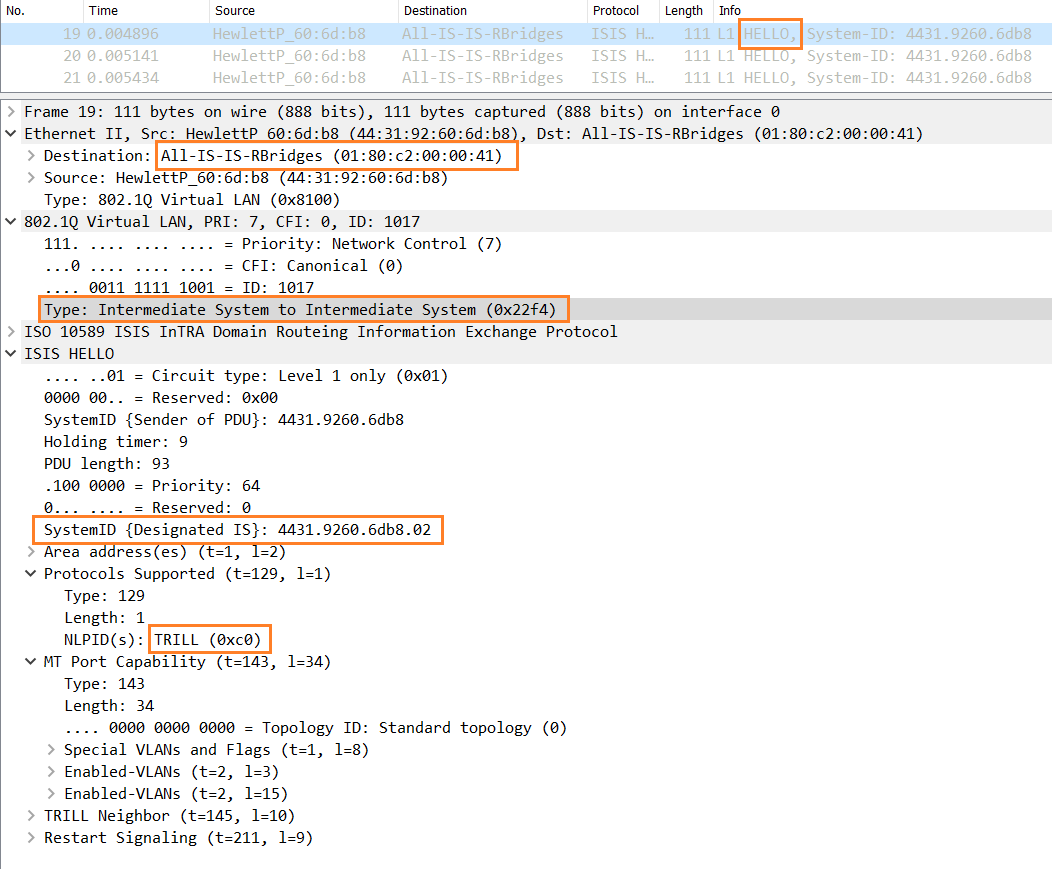
\includegraphics[width=\linewidth]{images/is_is_hello}
		\caption{IS-IS LSP (Link State PDU)}
		\label{fig:isislinkstatepdu}
	\end{figure}
	\item[LSP (Link State PDU)] Transportiert netzwerktopologische Informationen sowie CLNP (Connectionless Network Protocol) Pakete. Diese werden periodisch an die All IS-IS RBridges Mac Adresse versandt.
	\begin{figure}[h]
		\centering
		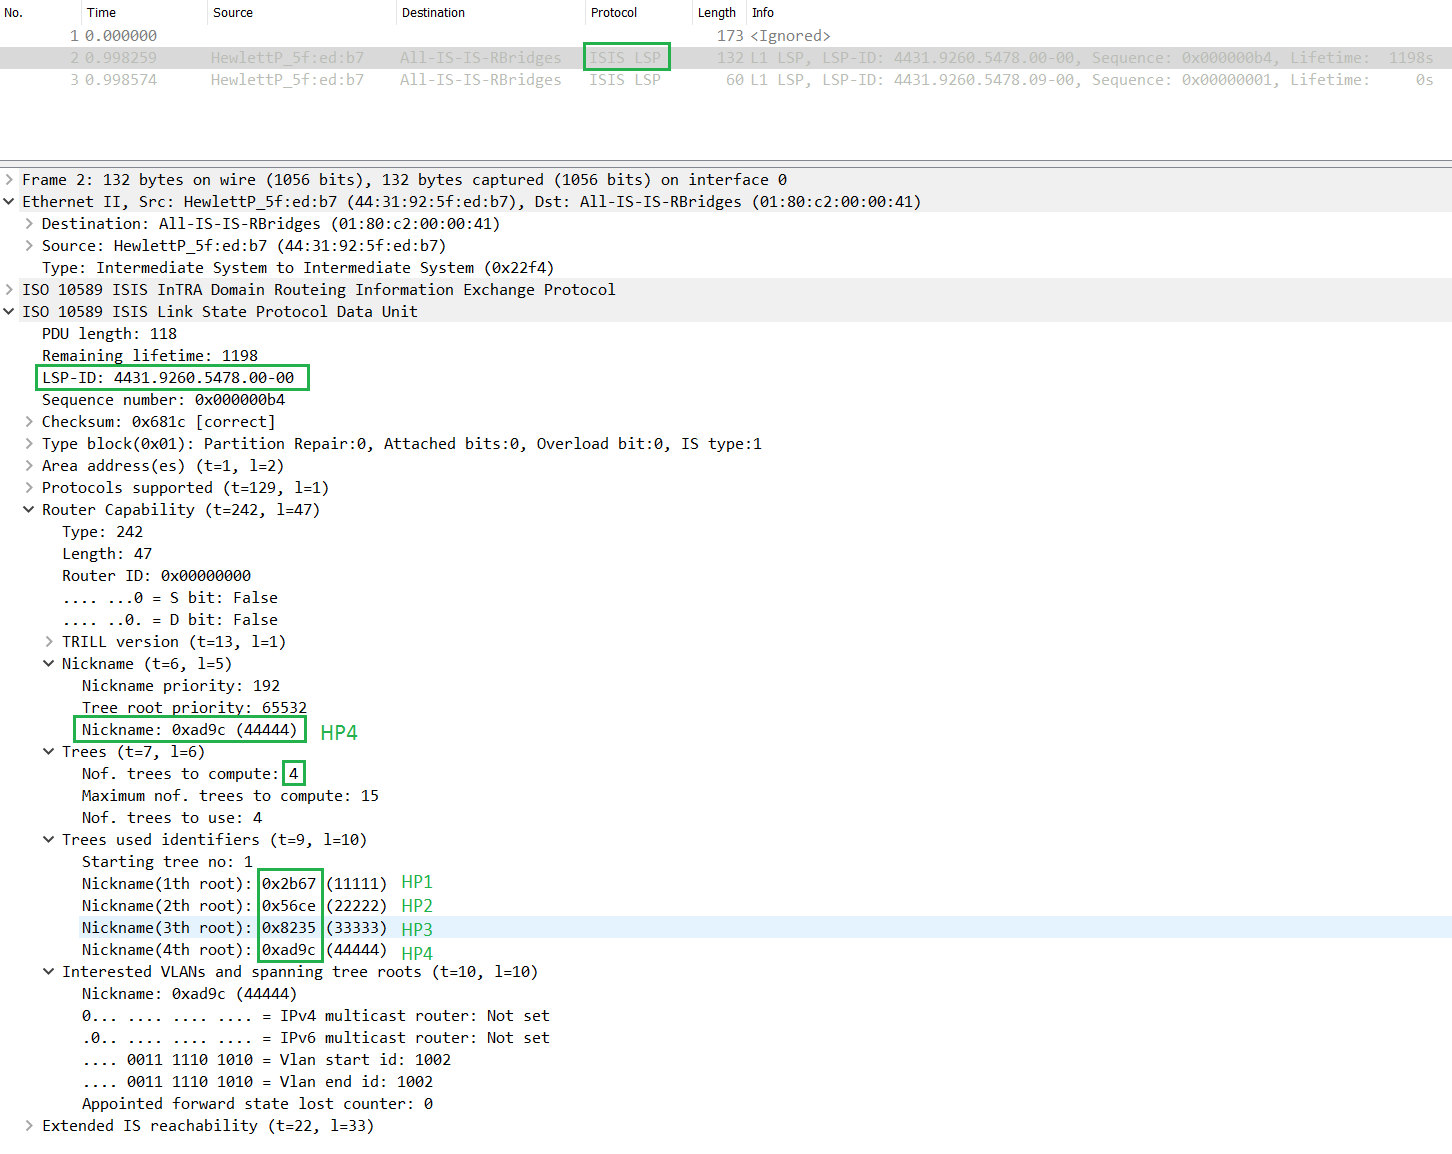
\includegraphics[width=\linewidth]{images/is_is_link_state_pdu}
		\caption{IS-IS LSP (Link State PDU)}
		\label{fig:isislinkstatepdu}
	\end{figure}
\end{description}

\clearpage


\subsubsection{Aufzeichnung Traffic}
Wir haben unserer Testumgebung gemäss der Abbildung \ref{fig:testaufbau} aufgebaut und auf alle Switches mit Wireshark gesnifft. Nach der Analyse der Wireshark Traces dokumierten wir den Paketaufbau, sowie das Verhalten von TRILL in der vorliegenden Dokumentation. 
\begin{figure}
	\centering
	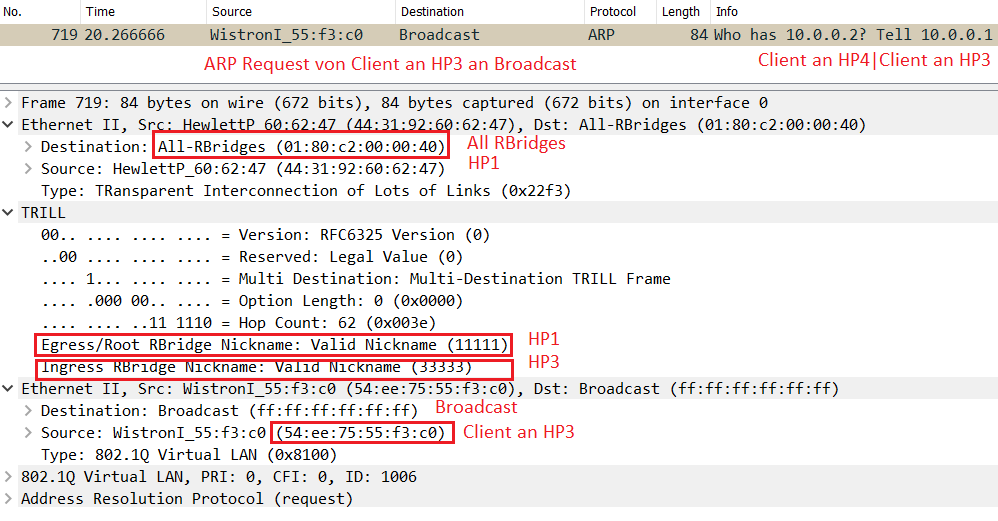
\includegraphics[width=\linewidth]{images/trill_package}
	\caption{ARP Request von Client A an Broadcast}
	\label{fig:trillpackage}
\end{figure}

\subsubsection{Trees: Multicast / Broadcast / Unknown Unicast}\label{sec:trees-multicast--broadcast--unknown-unicast}

Trees werden von TRILL mittels des Dijkstra Algorithmus von IS-IS mit den erhaltenen Geräte-Tree und damit bekannten Neighbors und Prioritäten aufgebaut. Die Nachbarn und Geräteprioritäten sind in der Tabelle und Grafik am Anfang des Kapitels \ref{sec:lab-konfiguration} ersichtlich.

Der Multicast-Tree steuert das verteilen von Multicast, ''Broadcast''\footnote{Ausserhalb des TRILL-Netzwerkes sind es MAC-Broadcast Pakete, innerhalb von TRILL werden sie als Multicast verteilt.} und Unknown-Unicast\footnote{Wenn die Ziel-MAC-Adresse dem Ingress-Switch noch nicht bekannt ist, verteilt er das Paket per Multicast an alle Egress-Switches}-Paketen im Netzwerk. Die Pakete werden jeweils entlang eines von einem Root aus gesehenen Tree verteilt; die Anzahl gewünschter Trees lässt sich im konfigurieren.

Die im Lab vorhandene TRILL-Konfiguration ist so konfiguriert, dass 4 Multicast Trees aufgebaut werden.

Die Struktur kann mit \lstinline|display trill multicast-route tree-root <NICK>| für einen Tree mit der Root beim Switch \lstinline|<NICK>| ausgelesen werden. Der jeweilige Switch leitet Pakete dann jeweils nach gemäss der Tree Struktur weiter. Der jeweils zu Verwendete Multicast Tree wird im ''Egress''-TRILL-Header definiert (siehe Abbildung \ref{fig:trillheadermulticast})

\begin{figure}[H]
\centering
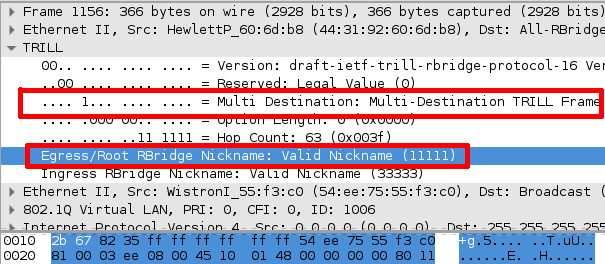
\includegraphics[width=0.7\linewidth]{images/trill_header_multicast}
\caption{TRILL Multicast-Header Felder}
\label{fig:trillheadermulticast}
\end{figure}


\paragraph{Fehler in Tree \lstinline|0x2b67|} \hfill \\
Im Tree \lstinline|0x2b67| (HP1) in Abbildung \ref{fig:multicasttree0x2b67} hat sich vermutlich einen Fehler eingeschlichen. Möglicherweise lässt sich dieser darauf zurückführen, dass ein Teil der Konfiguration (die auf HP3) erst eine Woche später aus den Switches ausgelesen wurde als die anderen und so ein inkonsistenter Zustand bzw. eine andere Treestruktur, z.B. aufgrund der Einschalt-Reihenfolge, ausgelesen wurde. Die entsprechenden Konfigurationen von \lstinline|0x2b67| sind:

\begin{lstlisting}
<HP1>display trill multicast-route tree-root 2b67
Root: 0x2b67
LocalRcvFlag: True
List of VLANs:
1003, 1006
List of outgoing ports:
XGE1/0/49
XGE1/0/50

<HP2>display trill multicast-route tree-root 2b67
Root: 0x2b67
LocalRcvFlag: True
List of VLANs:
1003, 1006
List of outgoing ports:
XGE1/0/50

[HP3]display trill multicast-route tree-root 2b67
Root: 0x2b67
LocalRcvFlag: True
List of VLANs: None
List of outgoing ports:
XGE1/0/49

<HP4>display trill multicast-route tree-root 2b67
Root: 0x2b67
LocalRcvFlag: True
List of VLANs:
1003, 1006
List of outgoing ports:
XGE1/0/49
XGE1/0/50
\end{lstlisting}

\paragraph{Tree-Strukturen} \hfill \\
Damit lassen sich folgende Tree-Strukturen auslesen:
\begin{figure}[H]
	\centering
	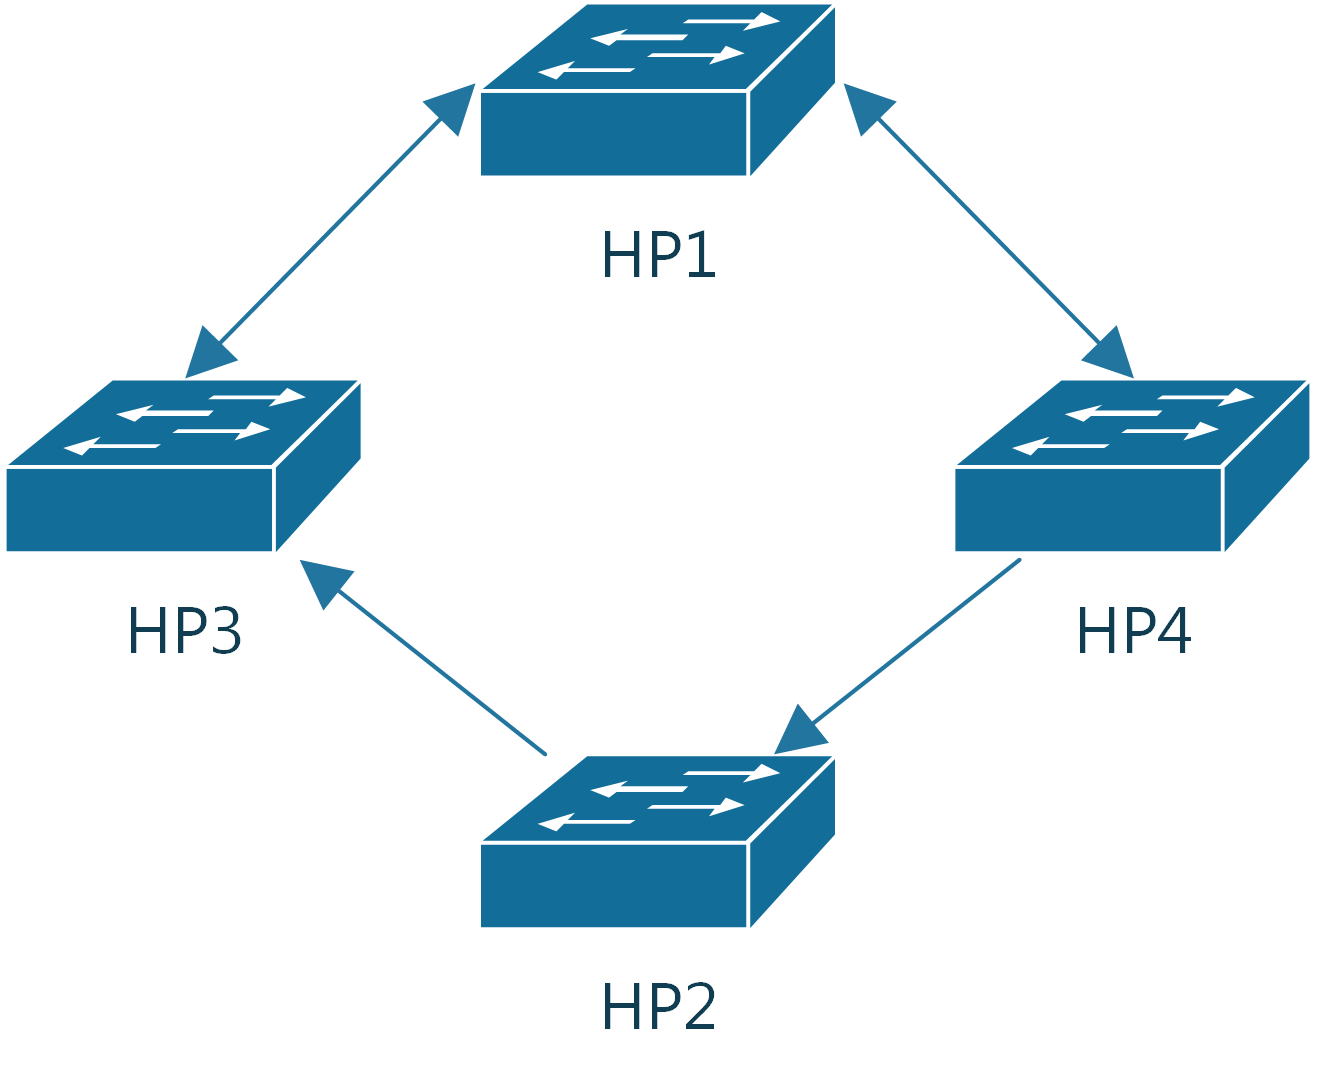
\includegraphics[width=0.5\linewidth]{images/multicast_trees/0x2b67}
	\caption{Multicast Tree Switch \lstinline|0x2b67| bzw. HP1. Hier ist vermutlich ein Fehler vorhanden (Siehe \ref{sec:trees-multicast--broadcast--unknown-unicast})}
	\label{fig:multicasttree0x2b67}
\end{figure}

\begin{figure}[H]
	\centering
	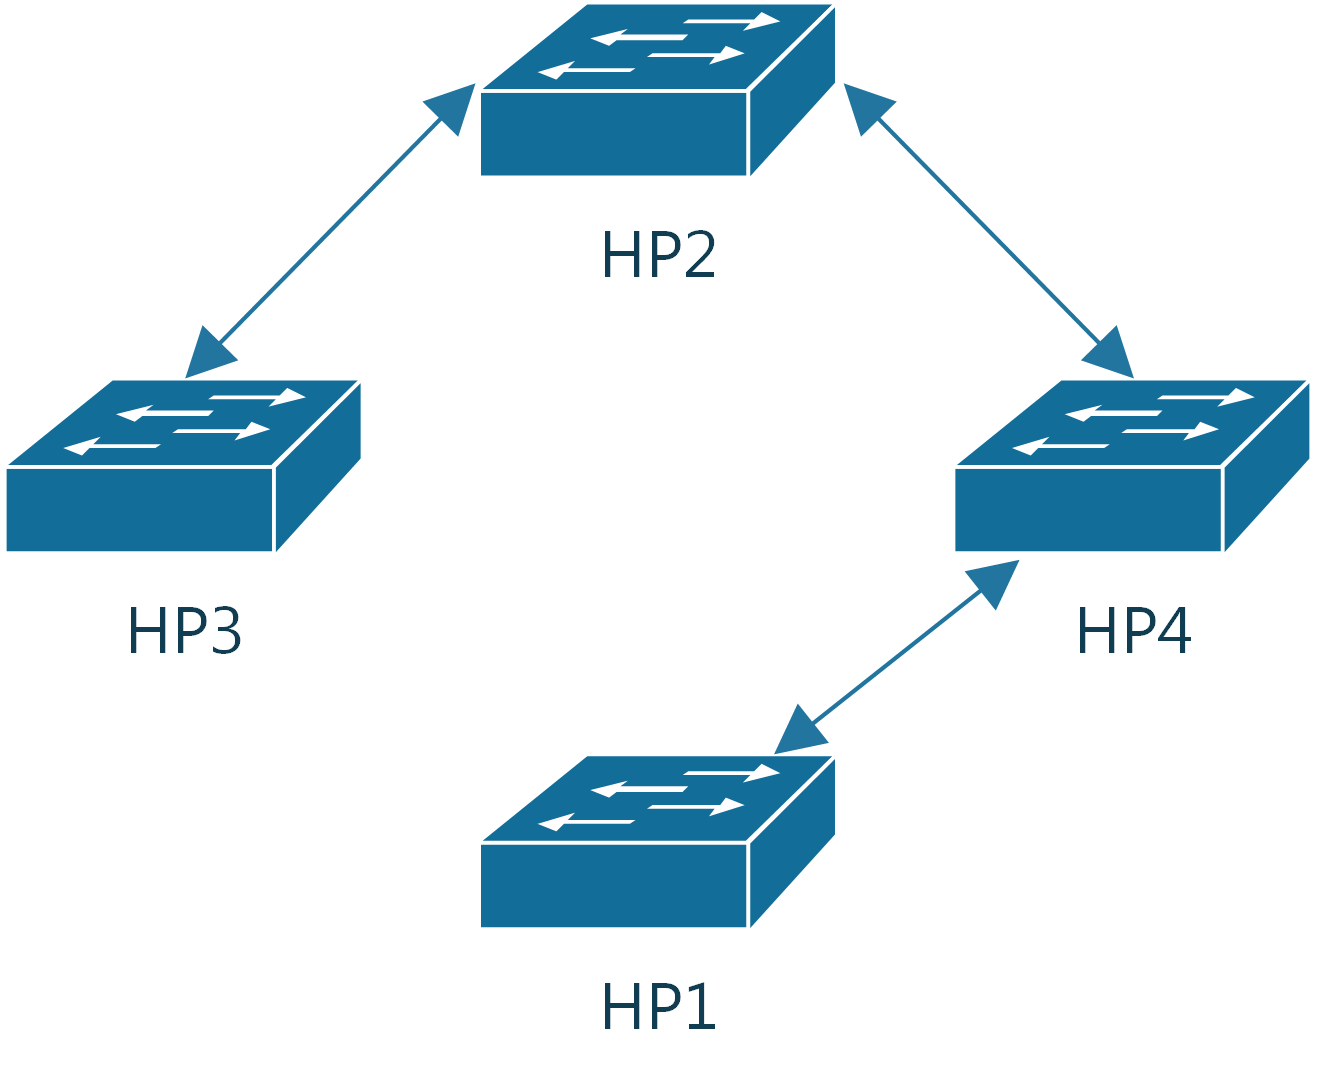
\includegraphics[width=0.5\linewidth]{images/multicast_trees/0x56ce}
	\caption{Multicast Tree Switch \lstinline|0x56ce| bzw. HP2}
	\label{fig:multicasttree0x56ce}
\end{figure}

\begin{figure}[H]
	\centering
	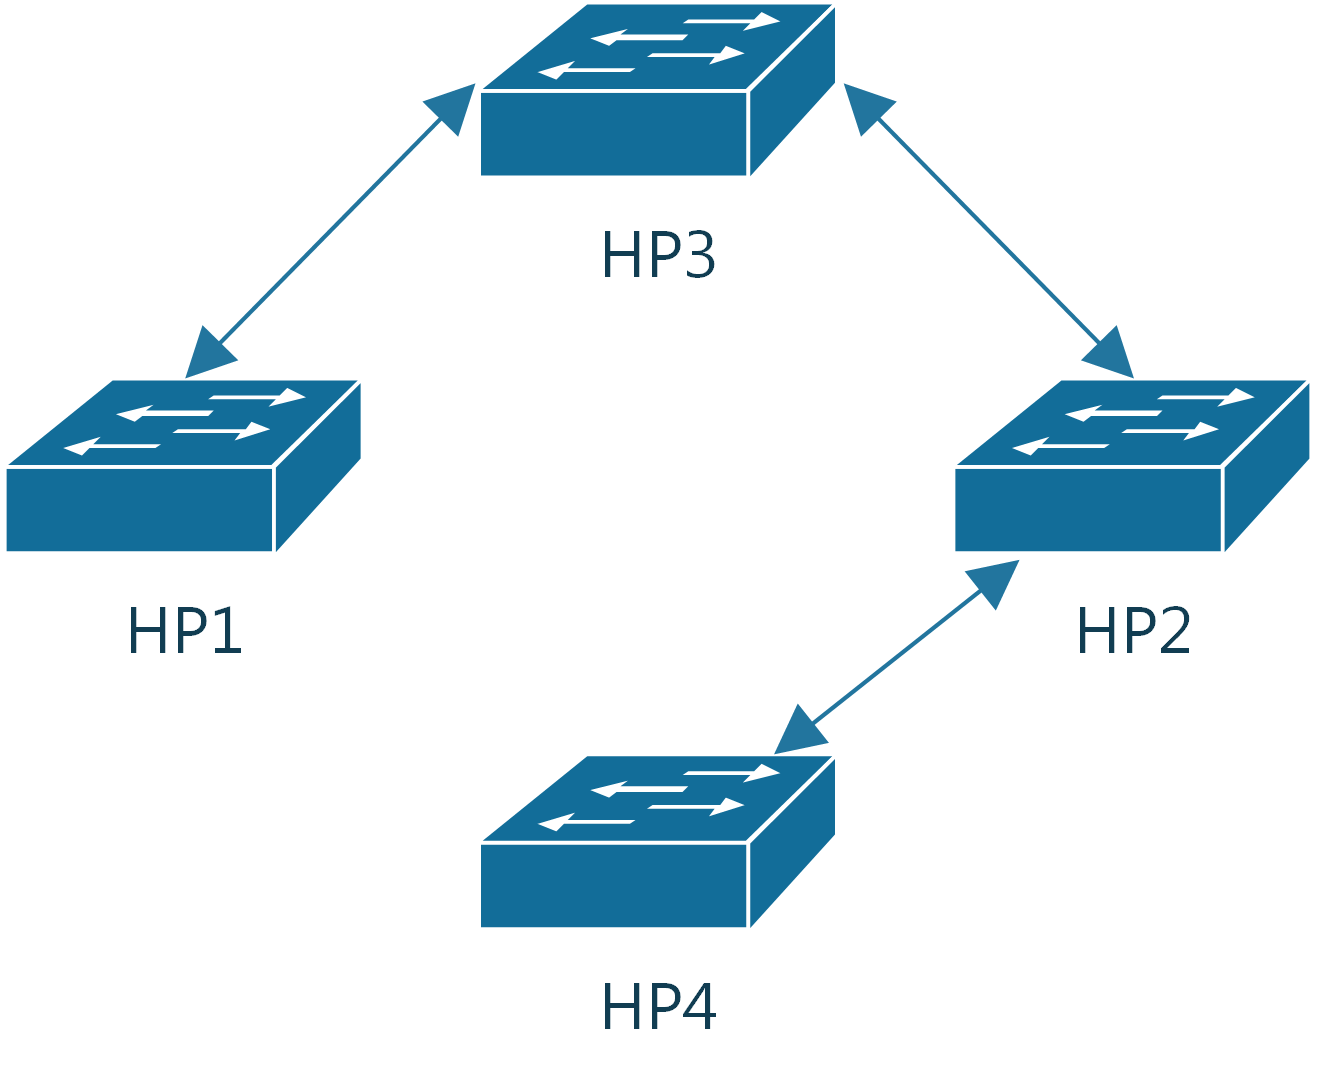
\includegraphics[width=0.5\linewidth]{images/multicast_trees/0x8235}
	\caption{Multicast Tree Switch \lstinline|0x8235| bzw. HP3}
	\label{fig:multicasttree0x8235s}
\end{figure}

\begin{figure}[H]
	\centering
	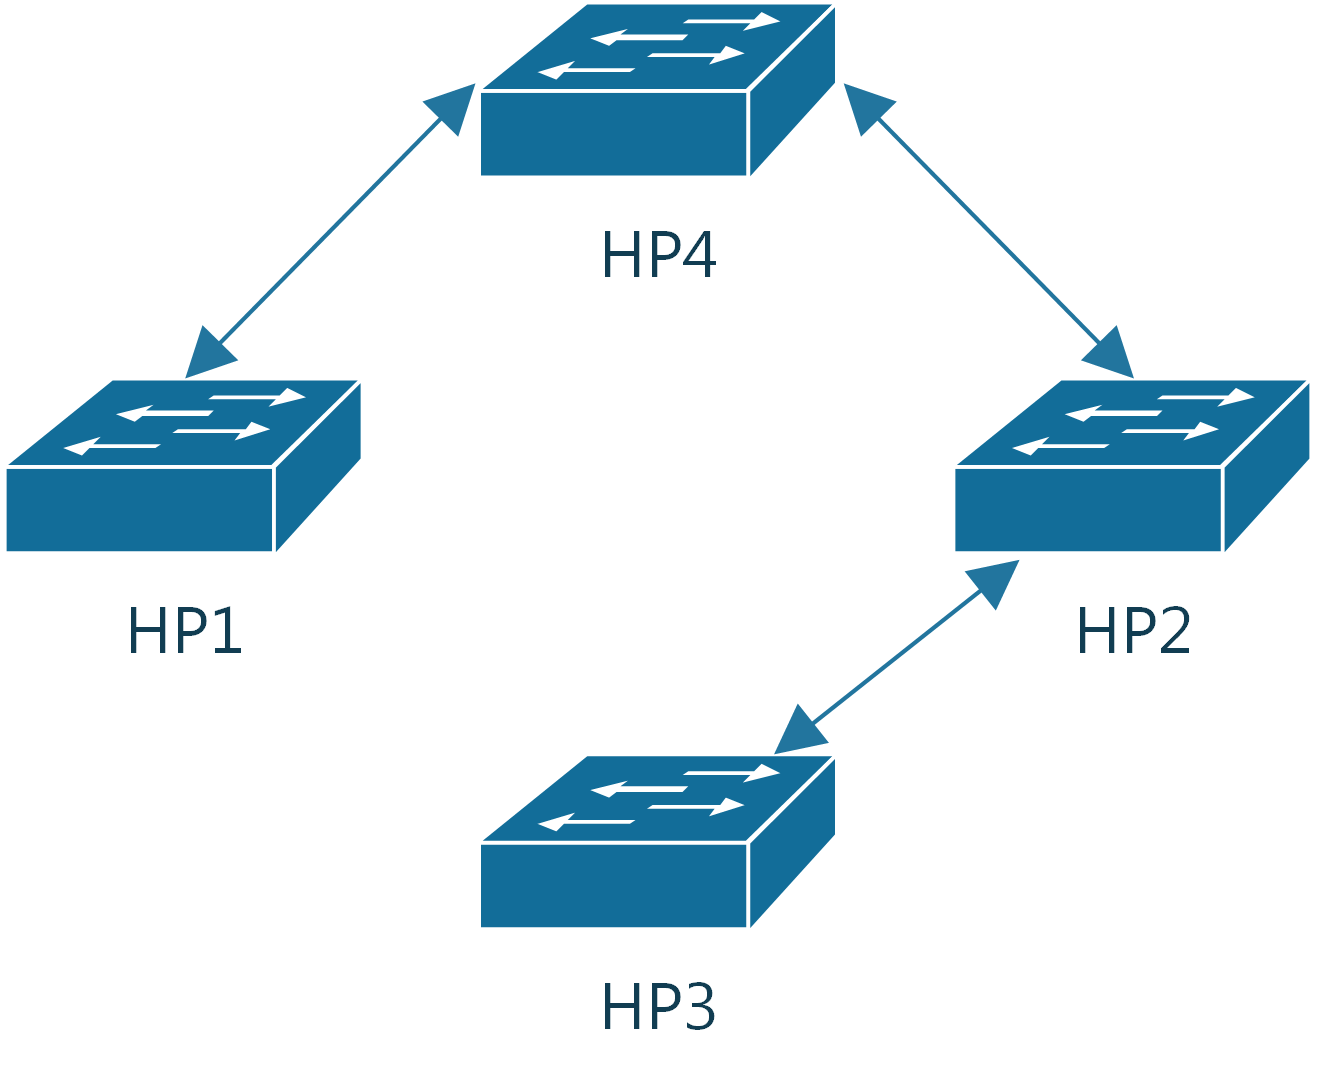
\includegraphics[width=0.5\linewidth]{images/multicast_trees/0xad9c}
	\caption{Multicast Tree Switch \lstinline|0xad9c| bzw. HP4}
	\label{fig:multicasttree0xad9c}
\end{figure}

\subsubsection{PacketFlow}
Bei TRILL unterscheided man zwischen zwei Varianten des Paketflusses:

\paragraph{Known Unicast} \hfill \\
Um die Egress Bridge zu bestimmen, wird bei Known Unicast Verkehr ein Lookup für die Ziel MAC-Adresse durchgeführt. Diese Information ist auf der Ingress Bridge aufgrund vorhergehender Kommunikation bereits bekannt. Anschliessend wird das Paket anhand des Egress Bridge Nicknames durch die Wolke weitergeleitet. Beim Ziel angekommen wird der TRILL Header entpackt und gemäss dem inneren Ethernet Header dem Empfänger zugestellt. Wenn zwei gleichwertige Pfade zur Verfügung stehen, wird ein Hash über die Source und Ziel MAC Adresse erstellt und dieser Modulo Portanzahl genommen. Die resultierende Zahl bestimmt die ausgehende Port Nummer.

Sind Empfänger und Sender dieselben, wird der Verkehr immer über das selbe Interface versendet.
\[
	M = H(MAC_{src}, MAC_{dest}) \text{ mod } N
\]
wobei 
\begin{itemize}[label={}]
	\item N = Anzahl verfügbare Ports
	\item M = Ausgehender Port
	\item H = Hash Funktion
\end{itemize}

 Wir konnten dieses Verhalten feststellen, als wir von Client A nach Client B einen Ping versendeten. Obschon HP3 zwei gleichwertige Pfade nach HP4 hat, wird immer der Pfad über HP2 verwendet.

\begin{figure}[H]
	\centering
	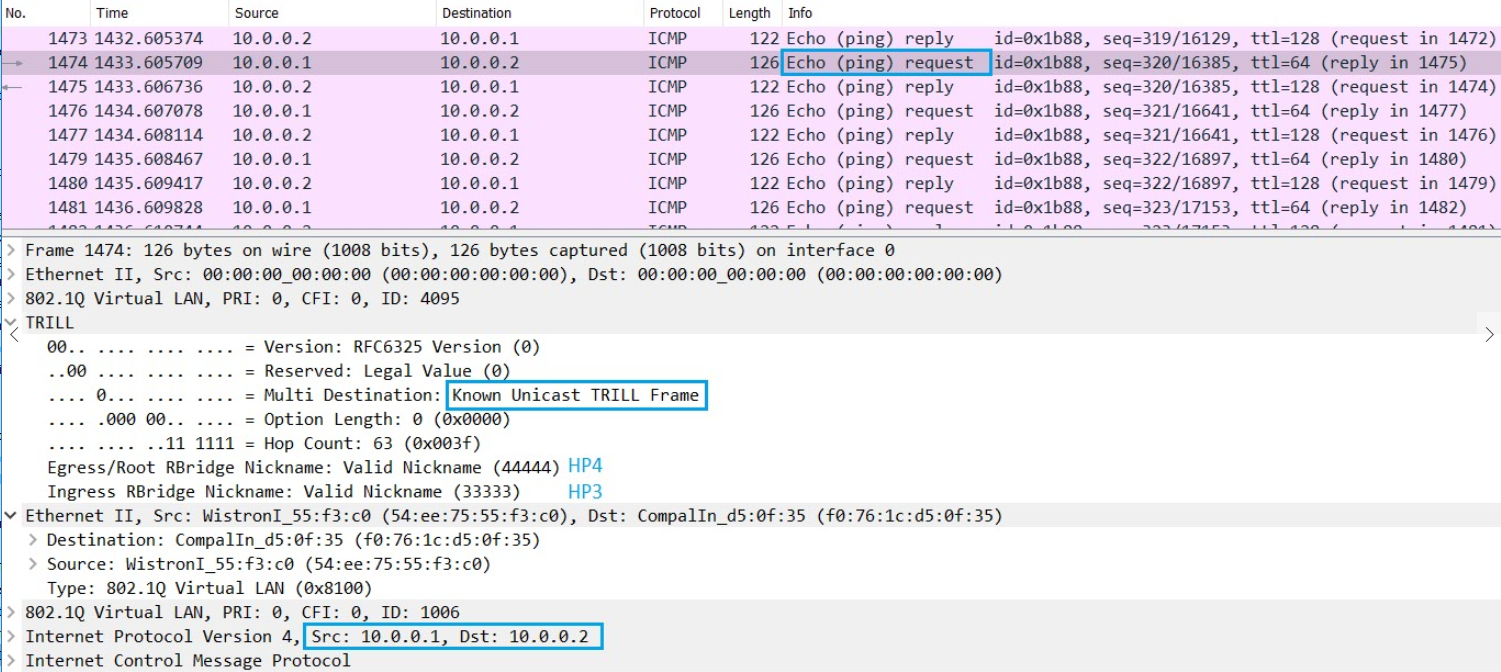
\includegraphics[width=\linewidth]{images/ping_request}
	\caption{Ping Request: Known Unicast TRILL Frame}
	\label{fig:trillpackage}
\end{figure}


\begin{figure}[H]
	\centering
	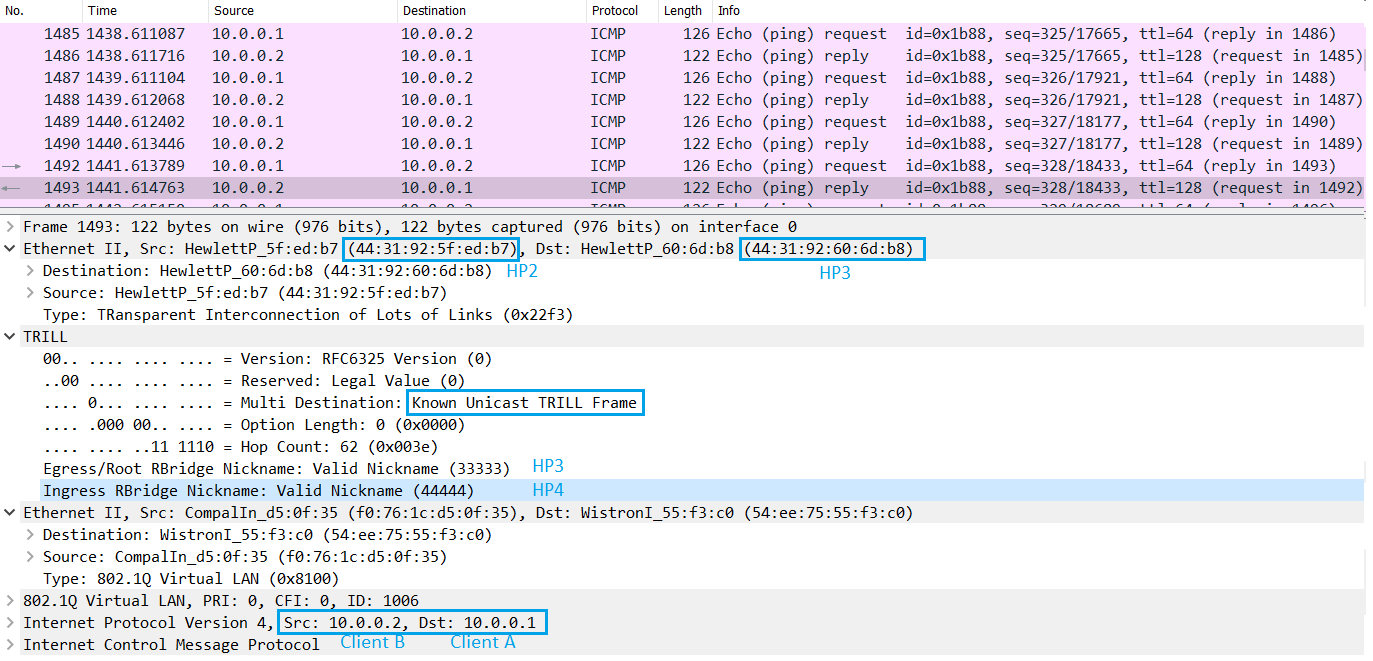
\includegraphics[width=\linewidth]{images/ping_reply}
	\caption{Ping Reply: Known Unicast TRILL Frame}
	\label{fig:trillpackage}
\end{figure}

\paragraph{Unknown Unicast, Broadcast, Multicast} \hfill \\
Geht der Verkehr an ein noch unbekanntes Ziel, wird das M-Bit gesetzt und das Paket entlang des Multicast Trees an alle Multicast Teilnehmer versendet. Beim Ziel angekommen wird der TRILL Header entfernt und an alle Teilnehmer gebroadcasted. Die Anwort zurück ist dann wieder Known Unicast. (\lstinline|ping|-reply) Zusätzlich lernen die RBridges bei diesem Vorgang die MAC Adressen, der angeschlossenen Clients (vergessen diese aber auch wieder nach wenigen Minuten, siehe Kapitel \ref{sec:mac-learning}).

\begin{figure}[H]
\centering
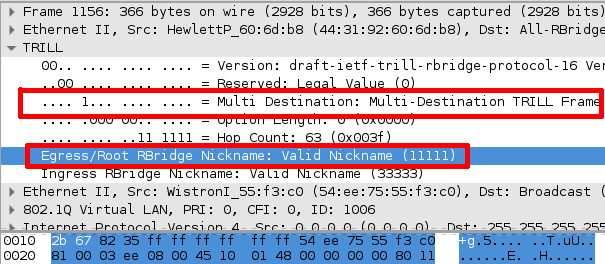
\includegraphics[width=0.7\linewidth]{images/trill_header_multicast}
\caption{TRILL Multicast Package}
\label{fig:trillheadermulticastpackage}
\end{figure}

\subsubsection{Mac Learning}\label{sec:mac-learning}
Die MAC Adressen werden grundsätzlich von den Edge Knoten gelernt.

TRILL lernt die MAC-Adressen, wie das für einen Switch gebräuchlich ist: Es merkt sich, auf welchen Ports Pakete von der MAC-Adresse eingegangen sind, und schickt Pakete an diese MAC-Adresse wiederum an diesen Port zurück. Diese Forwarding-Information wird allerdings nicht lange gespeichert, und meist nach kurzer Zeit wieder verworfen (üblicherweise 3 Minuten).

Kennt der Ingress-Switch die Destination-MAC-Adresse nicht, so verteilt er das Pakete gemäss dem hinterlegten Multicast-Tree (siehe auch Kapitel \ref{sec:trees-multicast--broadcast--unknown-unicast}).

Innerhalb der TRILL-Cloud werden Pakete mithilfe des ''Egress''-Headers weitergeleitet: Die MAC-Adresse des (inneren) Pakets spielt in der MAC-Cloud also keine Rolle mehr.

Wenn Geräte auf einem Switch eingesteckt werden, wird daher \textbf{nicht} die MAC Adresse via IS-IS verteilt; allerdings meldet IS-IS die Änderung eines Port-Zustandes mittels einer entsprechenden eindeutigen ID, welche sich auf den Switch und Switchport zurückführen lässt. So werden alle Switches über eine Änderung an den entsprechenden Geräten informiert; diese können als Reaktion darauf allenfalls ihre FIB anpassen.

\section{VXLAN}
\subsection{Terminologie}
\begin{description}
	\item[VXLAN: Virtual eXtensible Local Area Network] \hfill \\
	Ist ein Encapsulation Protokoll, um Overlay Netzwerke auf einer existierenden Layer 3 Infrastruktur umzusetzen.
	\item[VNI: VXLAN Network Identifier] \hfill \\
	24bit langer Identifiert pro VXLAN (vergleichbar mit VLAN Tag)
	\item[VTEP: VXLAN Tunnel End Point] \hfill \\
	Die ''externe'' IP Adresse des Virtuellen Switches. Der VTEP ist wie der Switch, teil der VM. Der VTEP enkapselt den VM Traffic in einem IP Header, damit dieser über ein Layer 3 Netzwerk gesendet werden kann. Die VM an sich verfügt über kein Wissen der VXLANs.
\end{description}

\subsection{Funktion}
VXLAN ist ein Overlay Protokoll, welches einem Host erlaubt, seine IP Adresse beizubehalten, obschon die VM ihren Standort gewechselt hat. Dies funktioniert, da der VTEP teil der VM ist und somit mitverschoben wird. Mittel VXLAN lassen sich logische Layer 2 Overlay Netzwerk auf das bestehende Layer 3 Netzwerk umsetzen. Die Layer 2 Pakete werden dann einfach in Layer 3 Header verpackt. Da in klassischen Netzes die MAC Broadcasts auf Layer 3 geblockt werden, muss das MAC Learning und Floading unter VXLAN mit Multicast emuliert werden. So wird Broadcast und Unknow-Unicast Verkehr einfach über Multicast übertragen. Bekannter Unicast Verkehr kann nach wie vor direkt übertragen werden. (gemäss Remote VTEP). Grundlegend läuft die Kommunikation wie folgt ab.

\begin{enumerate}
	\item VM1 möchte Daten Daten versenden und erstellt dafür ein L2 Ethernet Frame
	\item Das VXLAN Kernel Modul verpackt das Ethernet Frame in einem VXLAN Header, sowie einem UDP Header
	\item Ist die Ziel MAC Adresse in der Upstream Tabelle bereits bekannt, kann das Paket direkt an den Remote VTEP gesendet werden. Die entsprechenden Header werden hinzugefügt. Falls kein Mapping existiert, muss der ARP Broadcast, per Multicast an den Remote VTEP gesendet werden. Dieser entpackt das Paket und merkt sich das eingehende MAC-zu-VTEP Mapping. Die ARP Antwort kann dann per Unicast direkt zurück an den Sender gesendet werden.
\end{enumerate}

Damit der VXLAN Verkehr auf dem Weg nicht gedropt wird, muss eine minimale MTU von 1550Byte (empfohlen 1600Bytes) gesetzt werden. \\

Jeder VTEP speichert, welche MAC Adresse in welchem VXLAN über welchen Remote VTEP erreichbar ist, in einer eigenen Tabelle. Ebenfalls werden eingehende Pakete gemäss ihrer VNI wieder auf das korrekte VLAN gemappt.

\begin{table}[H]
	\centering
	\begin{tabu} to \linewidth {l l l}
		\toprule
		Mac Adresse & VNI & Remote VTEP \\
		\midrule
		\lstinline|01-01-01-01-01-01| & 1001 & 10.1.1.1 \\
		\lstinline|02-02-02-02-02-02| & 1002 & 10.1.1.2 \\
		\lstinline|03-03-03-03-03-03| & 1003 & 10.1.1.3 \\
		\bottomrule
	\end{tabu}
	\label{tbl:Lab devices}
	\caption{Upstream Table}
\end{table}

\begin{table}[H]
	\centering
	\begin{tabu} to \linewidth {l l}
		\toprule
		VLAN & VNI \\
		\midrule
		100 & 1001 \\
		200 & 1002 \\
		300 & 1003 \\
		\bottomrule
	\end{tabu}
	\label{tbl:Lab devices}
	\caption{Downstream Table}
\end{table}

\subsection{Protokoll Header}
Ein VXLAN Frame ist in fünf Schichten aufgeteilt:
\begin{description}
	\item[Outer Ethernet Header] \hfill \\
	Source und Destination MAC Adressen zwischen den VXLAN Lab Switches
	\item[Outer Ip Header] \hfill \\
	Der äussere IP Header beinhaltet die Source IP des eigenen VTEP, sowie die Destination IP des Remote VTEP. Im Lab waren dies \lstinline|vxlan-lab-sw01| und \lstinline|vxlan-lab-sw03|.
	\item[UDP Header] \hfill
	\begin{itemize}
		\item Source Port: Hash über den inneren Ethernet Header
		\item Destination Port: Default VXLAN Port 4789
	\end{itemize}
	\item[VXLAN Header] \hfill
	\begin{itemize}
		\item 8 Flag Bits: Das I Flag definiert ob der Header eine valid VXLAN ID hat. Die Restlichen Bits sind ''reserved'' und standardmässig auf 0 gesetzt.
		\item VNI: 24 Bit langer Identifier für ein VXLAN (vergleichbar mit VLAN)
	\end{itemize}
	\item[Inner Ethernet Header] \hfill \\
	Source und Destination MAC Adressen der beiden Clients/VM's
\end{description}

\begin{figure}[h]
	\centering
	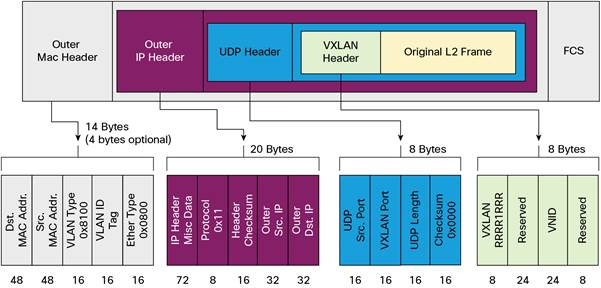
\includegraphics[width=0.8\linewidth]{images/vxlan_header}
	\caption{Logische Toplogie}
	\label{fig:vxlanheader}
\end{figure}
\clearpage

\begin{figure}[H]
	\centering
	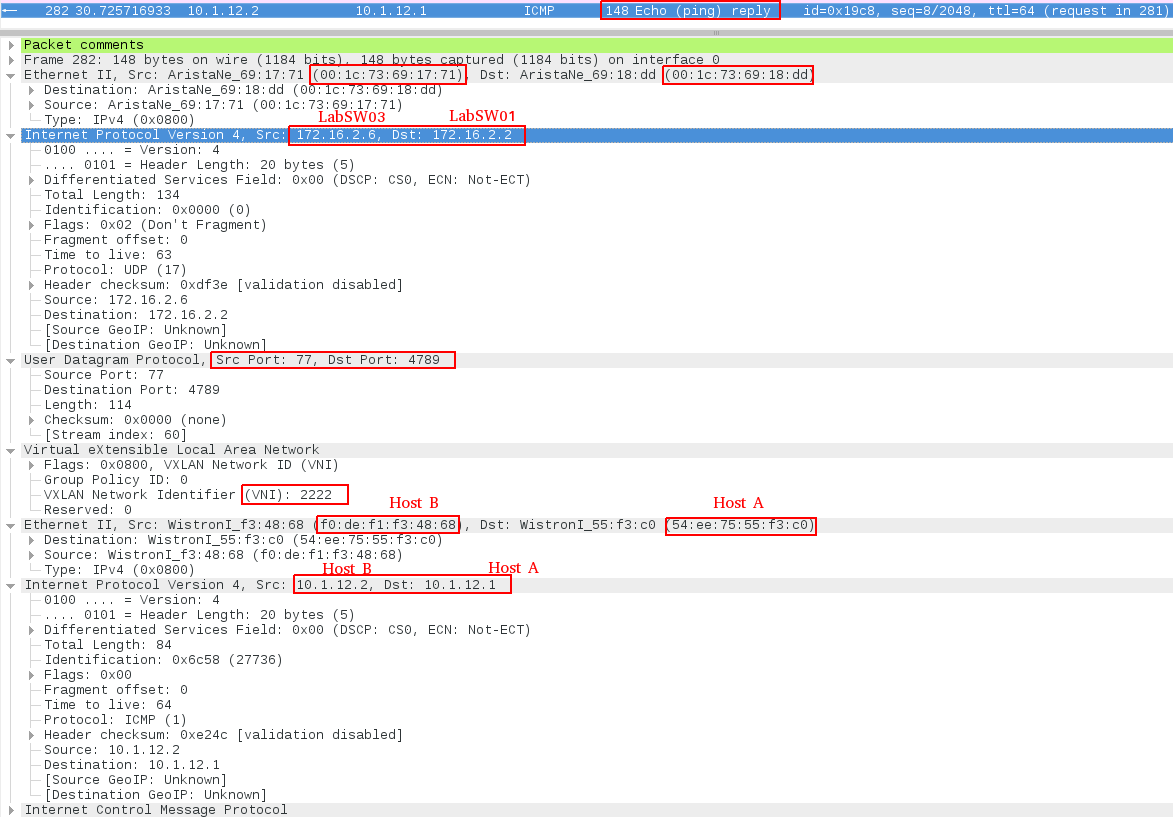
\includegraphics[width=0.8\linewidth]{images/ping_replay}
	\caption{Ping Reply Wireshark Trace}
	\label{fig:pingreply}
\end{figure}

\begin{figure}[H]
	\centering
	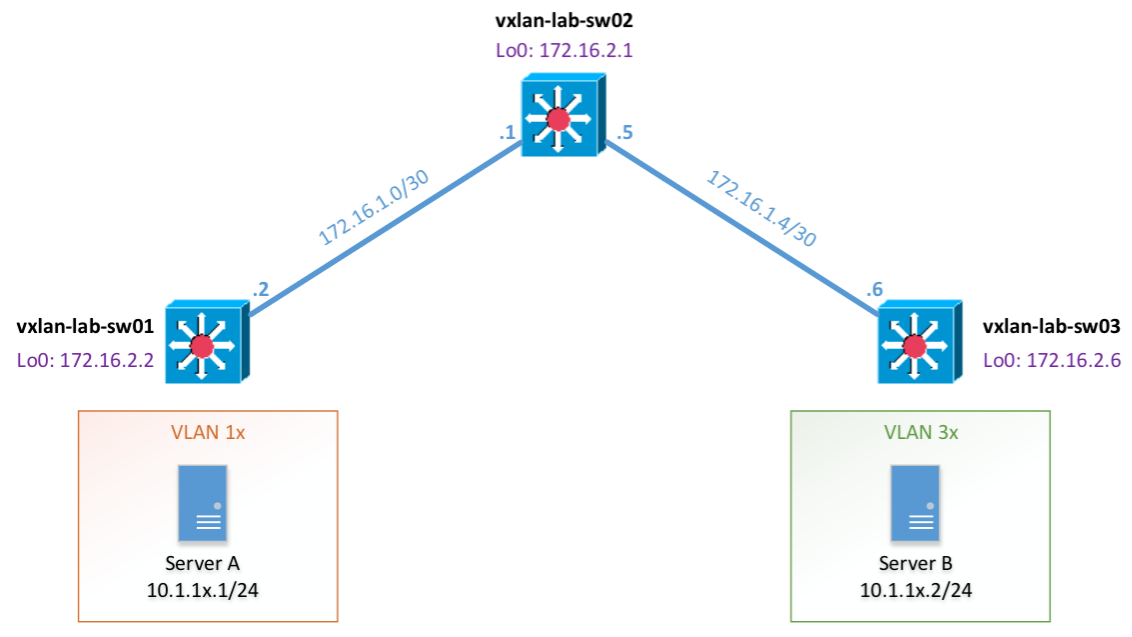
\includegraphics[width=0.6\linewidth]{images/vxlan_logical}
	\caption{Logische Umgebung im Lab}
	\label{fig:vxlanlogical}
\end{figure}
\newpage

\subsection{Ziel von VXLAN}
Traditionelle Datacenter Technologien haben einige Einschränkungen und können den Ansprüchen moderener Datencenter nicht mehr gerecht werden. 
\begin{itemize}
	\item Für die Aufteilung des Traffics in einem mandantenfähigen System, sind mehr als 4096 VLANs nötig
	\item Durch Virtualisierung braucht jede VM eine eindeutige MAC Adresse. Dies bedeutet, dass die Kapazität der MAC Adresstabelle um ein vielfaches wachsen müsste. 
	\item STP blockiert die redundanten Links, damit keine Loops entstehen. Dies erschwert den Einsatz von ECMP, obschon der Einsatz von ECMP auf Layer 3 einfach umzusetzen ist. Gefragt ist die Funktionalität jedoch auf Layer 2
\end{itemize}
VXLAN geht genau diese Probleme an. Mit VXLAN können Layer 2 Overlay Netze auf dem bestehenden Layer 3 Netz betrieben werden. Durch den Einsatz der 24 Bit VNI, stehen genügend logische Netze zur Verfügung, damit auch grosse Cloud Anbieter ihre Mandanten sauber trennen können. 


\subsection{Warum wurde VXLAN entwickelt}
VXLAN wurde primär entwickelt, um VLAN zu erweitern. Da VLAN auf 4096 logische Netze (12Bit) eingeschränkt ist, hat man die VNI unter VXLAN auf 24 Bit erweitert. Dies erlaubt 16'777'216 logische Netzwerke. Daher, mit VXLAN lassen sich $\approx$ 16 Millionen isolierte Layer 2 Netzwerke auf einer bestehenden Layer 3 Infrasturktur betreiben, welche intern wieder 4096 VLAN's enthalten können. VXLAN wurde usprünglich von Cisco, VMware und Arista Networks entwickelt. 

\subsection{Wo und wie kann VXLAN eingesetzt werden (Use Cases)}

Der Einsatz von VXLAN macht Sinn, wenn ein über mehrere physiche Hosts verteiltes, virtuelles Netzwerk mit vielen Segmenten und viel Traffic existieren soll, wie dies in einem grösseren Datacenter üblicherweise der Fall ist. Das zugrundeliegende ''physische'' Netzwerk sollte ein geroutetes Netzwerk sein, damit VXLAN einen entsprechenden Vorteil bring.

Auf der virtuellen Umgebung ist es nötig, virtuelle Switches zu erstellen, welche das verpacken und routen der Pakete vornehmen. Dies kann entweder durch den Einsatz entsprechender virtueller oder physischer Maschinen erfolgen, oder über eine Native Unterstützung der Umgebung. Zusätzlich braucht es entsprechende Gateways zwischen physichen und virtuellen Netzwerken.

\subsection{Ist VXLAN kompatibel mit traditionellen Protokollen}
% If yes, what are the differences and which limitations does VXLAN solve?

VXLAN ist kompatibel mit ''traditionellen'' Protokollen wie VLAN, da die Pakete eins zu eins wiederum in UDP eingepackt werden, ohne gross Veränderungen vorzunehmen. 

VXLAN wurde zudem so entwickelt, dass die bestehende L2 und L3 Infrastruktur weiter genutzt werden kann (abgesehen von den (meist virtuellen) Edge-Switches, welche eben das VXLAN verpacken/entpacken müssen). Das heisst, VXLAN arbeitet komplett im (tatsächlichen) Layer 3 und höher.

Die Zentrale Einschränkung von traditionellen Protokollen ist ebenfalls, dass diese nicht zwischen dem ''Wo'' und ''Wer'' unterscheiden. Mit VXLAN gibt es neben einem ''Wer'' (die MAC-Adresse) und ein ''Wo'' (die IP-Adresse) ein Overlay Netzwerk, welches das ''Wo'' weiter von der (VM- oder Container-)IP-Adresse abstrahiert.

\subsubsection{Vergleich mit VLAN}

Im Vergleich zu VLANs erfüllt VXLAN eine etwas etwas andere Funktion; es ermöglicht noch deutlich grössere Netzwerke und, der wohl wichtigste Unterschied: Es Routet die Pakete und verteilt L2-Broadcasts über Multicast. Damit erübrigt sich der Einsatz von z.B. STP, was zu einer verbesserten Performance und Durchsatz führt.

\subsubsection{Vergleich mit TRILL}

Im vergleich zu TRILL (welches im Kapitel \ref{sec:trill} bereits ausführlich behandelt wurde), setzt VXLAN stärker auf ein ''Tunneling''/ Layer 3-Konzept, welches mehr auf virtuelle Umgebungen ausgelegt ist. Layer 2 / TRILL trennt in diesem Sinne die Identität und den Ort.

Layer 3 bringt dafür einige Vorteile mit sich, unter anderem:

\begin{itemize}
	\item besser Skalierbar
	\item bessere Mobilität
	\item einfacheres Handling von Adressen/Identitäten
	\item Integrierte Möglichkeit von Routing und damit Ausnutzung der ganzen Bandbreite
	\item Effizientere Verknüpfung von Netzwerken
	\item Keine Broadcasts
\end{itemize}

\subsection{Was sind die Vor- und Nachteile von VXLAN}

\paragraph{Vorteile}
\begin{itemize}
	\item Benötigt keine spezielle Hardware, da die Übertragung via klassischem IP erfolgt
	\item Kann bis zu 16 Millionen logische Netzwerke verwalten (24 Bit Identifier)
	\item Die VMs bemerken von VXLAN nichts (handling auf dem (v)Switch).
	\item Braucht keinen zentralen Controller
	\item Tunnelt die virtuellen Hosts
	\item Die VMs / Container sind damit ''mobil'' und können ohne Probleme verschoben werden.
\end{itemize}

\paragraph{Nachteile}
\begin{itemize}
	\item Der Overhead ist aufgrund der grossen Verschachtelung relativ gross (ca. 50Bytes pro Paket)
	\item Die Latenz wird aufgrund des Ein- und Auspacken grösser und braucht mehr Rechenleistung.
	\item Der ganze L3-Traffic (wie ARP etc.) muss über ''langsame'' L3-Devices an viele Orte verteilt werden.
	\item Möglicherweise suboptimaler Traffic-Flow
	\item ECMP ist nicht zwingend garantiert
	\item Mehr Komplexität im Netzwerk
	\item Kein einheitlicher Herstellerstandard
	\item Keine einfache Integrationen anderer, phyischer Netzwerke bzw. Eingehenden Verkehrs.
	\item Keine Absicherung: Ein Gerät, welche sich im VXLAN-Netzwerk befindet, hat vollen Zugriff auf das ganze Netzwerk.
	\item Möglicherweise Paketverlust im Netzwerk (UDP)
	\item Aufgrund der grösseren Paketgrösse kann es bei suboptimaler Konfiguration von kleineren Netzwerk-MTUs zu IP-Fragmentierung kommen (<1550 Bytes bzw. VM MTU + mindestens 50 Bytes, besser + 100 Bytes für IPv6 und VLANs)
\end{itemize}

\subsection{Gibt es andere moderne Technologien, welche VXLAN ähnlich sind?}

Ja, es gibt noch mehrere ähnliche Protokolle verschiedener Hersteller. Hier eine kurze Übersicht über die verschiedenen Funktionen / Eigenschaften:

\begin{table}[h]
	\centering
	\begin{tabu} to \linewidth {r X X X X}
		\toprule
		& VXLAN & NVGRE & STT & GENEVE \\
		\midrule
		Summary
			& Host-Overlay Protokoll u.a. von VMWare
			& Host-Overlay Protokoll von Microsoft
			& Host-Overlay Protokoll u.a. von VMWare
			& Tunneling-Only Protokoll \\
		Adresslänge & 24b & 24b & 64b & 24b \\
		Overhead & 56B & 46B & 80B & 54+B \\
		Verpackung & UDP & GRE & TCP & UDP \\
		Support & VMWare, Cisco, Arista & Microsoft, Arista & VMWare, Broadcom & VMWare, Microsoft RedHat, Intel \\
		Signaling & Flood \& Learn & Control Plane & Controller-based & (Tunnel only) \\
		Stärken & Weit verbreitet & Guter Microsoft-Support & Verlustfreie Übertragung & Nur Tunnelling \\
		Schwächen & Standardmässig kein Controller, dadurch mehr Traffic & z.T. fehlende Unterstützung, braucht spezielle Hardware & Viel Overhead \& Latenz durch TCP & Nur Tunneling \\
		\bottomrule
	\end{tabu}
	\label{tbl:VXLANcompare}
	\caption{Vergleich zwischen VXLAN und ähnlichen Technologien}
\end{table}


\subsection{Lab Konfiguration}
Es wurde folgende logische Topologie in zwei virtuellen Ubuntu Maschinen abgebildet. Die dazu nötigen Schritte konnten ohne Probleme ausgeführt werden. Innerhalb der beiden virtuellen Maschinen wurde je ein Mininet mit je 4 virtuellen Hosts und einem Switch erstellt. Die Hosts können nur innerhalb des eigenen VLAN's kommunizieren. Die beiden virtuellen Switches verfügen über einen VTEP und erlauben die VM-übergreifende Kommunikation. Nachdem der VNI auf das korrekte VLAN und Remote VTEP gemappt wurde, war die Kommunikation zwischen den Mininets ohne Probleme möglich.

\begin{figure}[h]
\centering
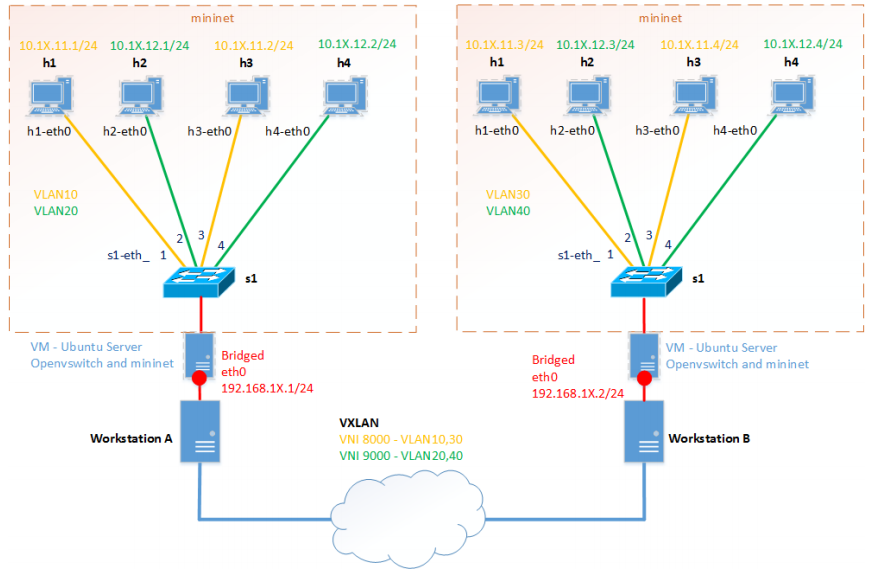
\includegraphics[width=0.7\linewidth]{images/vxlan_overview}
\caption{Logische Toplogie}
\label{fig:vxlanoverview}
\end{figure}

In einem ersten Schritt wurde die Konfiguration der VLAN's getestet (\lstinline|pingall|). Die virtuellen Host dürfen wie in der Abbildung ersichtlich, nur auf die Hosts im selben VLAN zugreifen.

\begin{figure}[h]
\centering
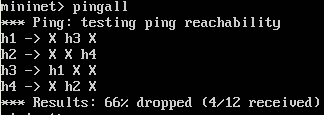
\includegraphics[width=0.5\linewidth]{images/vxlan_vlan_pingall}
\caption{VLAN Test durch Pingall}
\label{fig:vxlanvlanpingall}
\end{figure}
\newpage

In einem zweiten Schritt wurde dann die abgeschlossenen VXLAN Konfiguration getestet.
\begin{itemize}
	\item Mininet links: \lstinline|h1 ping 10.12.11.3| $\rightarrow$ Wie erwartet erfolgreich
	\item Mininet links: \lstinline|h2 ping 10.12.11.3| $\rightarrow$ Wie erwartet, keine Verbindung
	\item Mininet links: \lstinline|h2 ping 10.12.12.3| $\rightarrow$ Wie erwartet erfolgreich
\end{itemize} 
\begin{figure}[h]
	\centering
	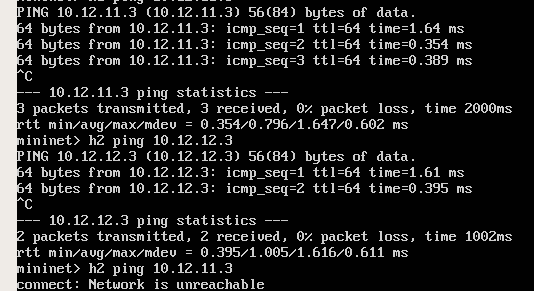
\includegraphics[width=0.5\linewidth]{images/vxlan_final_test.png}
	\caption{VLAN Test durch Pingall}
	\label{fig:vxlanvlanpingall}
\end{figure}

\appendix

\section{Konfigurationen}
\label{appendix:configurations}

\subsection{BR1-R1}
\subsubsection{Running Configuration}
\lstinputlisting{appendix/config/br1-r1/br1-r1-config.txt}

\subsubsection{IP Interfaces}
\lstinputlisting{appendix/config/br1-r1/br1-r1-interface.txt}

\subsubsection{Interface Status}
\lstinputlisting{appendix/config/br1-r1/br1-r1-status.txt}

\subsubsection{Neighbors}
\lstinputlisting{appendix/config/br1-r1/br1-r1-neighbors.txt}

\subsection{BR2-R1}
\subsubsection{Running Configuration}
\lstinputlisting{appendix/config/br2-r1/br2-ri-config.txt}

\subsubsection{IP Interfaces}
\lstinputlisting{appendix/config/br2-r1/br2-ri-interface.txt}

\subsubsection{Interface Status}
\lstinputlisting{appendix/config/br2-r1/br2-ri-status.txt}

\subsubsection{Neighbors}
\lstinputlisting{appendix/config/br2-r1/br2-ri-neighbors.txt}

\subsection{BR2-S1}
\subsubsection{Running Configuration}
\lstinputlisting{appendix/config/br2-s1/br2-s1-config.txt}

\subsubsection{IP Interfaces}
\lstinputlisting{appendix/config/br2-s1/br2-s1-interface.txt}

\subsubsection{Interface Status}
\lstinputlisting{appendix/config/br2-s1/br2-s1-status.txt}

\subsubsection{Neighbors}
\lstinputlisting{appendix/config/br2-s1/br2-s1-neighbors.txt}

\subsection{CCNA-CCNP-FRSwitch}
\subsubsection{Running Configuration}
\lstinputlisting{appendix/config/framerelayswitch/framerelayswitch-config.txt}

\subsubsection{IP Interfaces}
\lstinputlisting{appendix/config/framerelayswitch/framerelayswitch-interface.txt}

\subsubsection{Interface Status}
\lstinputlisting{appendix/config/framerelayswitch/framerelayswitch-status.txt}

\subsubsection{Neighbors}
\lstinputlisting{appendix/config/framerelayswitch/framerelayswitch-neighbors.txt}

\subsection{HQ FrameRelay Router (HQ-FRR)}
\subsubsection{Running Configuration}
\lstinputlisting{appendix/config/hq-frr/hq-frr-config.txt}

\subsubsection{IP Interfaces}
\lstinputlisting{appendix/config/hq-frr/hq-frr-interface.txt}

\subsubsection{Interface Status}
\lstinputlisting{appendix/config/hq-frr/hq-frr-status.txt}

\subsubsection{Neighbors}
\lstinputlisting{appendix/config/hq-frr/hq-frr-neighbors.txt}

\subsection{HQ-IER1}
\subsubsection{Running Configuration}
\lstinputlisting{appendix/config/hq-ier1/hq-ier1-config.txt}

\subsubsection{IP Interfaces}
\lstinputlisting{appendix/config/hq-ier1/hq-ier1-interface.txt}

\subsubsection{Interface Status}
\lstinputlisting{appendix/config/hq-ier1/hq-ier1-status.txt}

\subsubsection{Neighbors}
\lstinputlisting{appendix/config/hq-ier1/hq-ier1-neighbors.txt}

\subsection{HQ-WER1}
\subsubsection{Running Configuration}
\lstinputlisting{appendix/config/hq-wer1/hq-wer1-config.txt}

\subsubsection{IP Interfaces}
\lstinputlisting{appendix/config/hq-wer1/hq-wer1-interface.txt}

\subsubsection{Interface Status}
\lstinputlisting{appendix/config/hq-wer1/hq-wer1-status.txt}

\subsubsection{Neighbors}
\lstinputlisting{appendix/config/hq-wer1/hq-wer1-neighbors.txt}

\subsection{HQ CS1}
\subsubsection{Running Configuration}
\lstinputlisting{appendix/config/hq-cs1/hq-cs1-config.txt}

\subsubsection{IP Interfaces}
\lstinputlisting{appendix/config/hq-cs1/hq-cs1-interface.txt}

\subsubsection{Interface Status}
\lstinputlisting{appendix/config/hq-cs1/hq-cs1-status.txt}

\subsubsection{Neighbors}
\lstinputlisting{appendix/config/hq-cs1/hq-cs1-neighbors.txt}

\subsection{HQ CS2}
\subsubsection{Running Configuration}
\lstinputlisting{appendix/config/hq-cs2/hq-cs2-config.txt}

\subsubsection{IP Interfaces}
\lstinputlisting{appendix/config/hq-cs2/hq-cs2-interface.txt}

\subsubsection{Interface Status}
\lstinputlisting{appendix/config/hq-cs2/hq-cs2-status.txt}

\subsubsection{Neighbors}
\lstinputlisting{appendix/config/hq-cs2/hq-cs2-neighbors.txt}

\subsection{HQ CS3}
\subsubsection{Running Configuration}
\lstinputlisting{appendix/config/hq-cs3/hq-cs3-config.txt}

\subsubsection{IP Interfaces}
\lstinputlisting{appendix/config/hq-cs3/hq-cs3-interface.txt}

\subsubsection{Interface Status}
\lstinputlisting{appendix/config/hq-cs3/hq-cs3-status.txt}

\subsubsection{Neighbors}
\lstinputlisting{appendix/config/hq-cs3/hq-cs3-neighbors.txt}

\subsection{HQ CS4}
\subsubsection{Running Configuration}
\lstinputlisting{appendix/config/hq-cs4/hq-cs4-config.txt}

\subsubsection{IP Interfaces}
\lstinputlisting{appendix/config/hq-cs4/hq-cs4-interface.txt}

\subsubsection{Interface Status}
\lstinputlisting{appendix/config/hq-cs4/hq-cs4-status.txt}

\subsubsection{Neighbors}
\lstinputlisting{appendix/config/hq-cs4/hq-cs4-neighbors.txt}

\subsection{HQ DS1}
\subsubsection{Running Configuration}
\lstinputlisting{appendix/config/hq-ds1/hq-ds1-config.txt}

\subsubsection{IP Interfaces}
\lstinputlisting{appendix/config/hq-ds1/hq-ds1-interface.txt}

\subsubsection{Interface Status}
\lstinputlisting{appendix/config/hq-ds1/hq-ds1-status.txt}

\subsubsection{Neighbors}
\lstinputlisting{appendix/config/hq-ds1/hq-ds1-neighbors.txt}

\subsection{HQ DS2}
\subsubsection{Running Configuration}
\lstinputlisting{appendix/config/hq-ds2/hq-ds2-config.txt}

\subsubsection{IP Interfaces}
\lstinputlisting{appendix/config/hq-ds2/hq-ds2-interface.txt}

\subsubsection{Interface Status}
\lstinputlisting{appendix/config/hq-ds2/hq-ds2-status.txt}

\subsubsection{Neighbors}
\lstinputlisting{appendix/config/hq-ds2/hq-ds2-neighbors.txt}

\subsection{HQ DS3}
\subsubsection{Running Configuration}
\lstinputlisting{appendix/config/hq-ds3/hq-ds3-config.txt}

\subsubsection{IP Interfaces}
\lstinputlisting{appendix/config/hq-ds3/hq-ds3-interface.txt}

\subsubsection{Interface Status}
\lstinputlisting{appendix/config/hq-ds3/hq-ds3-status.txt}

\subsubsection{Neighbors}
\lstinputlisting{appendix/config/hq-ds3/hq-ds3-neighbors.txt}


\section{Messungen}
\label{appendix:measures}
\subsection{Von X nach Y}
\lstinputlisting{appendix/config/br2-r1/br2-ri-config.txt}

% Code Listings
% \lstlistoflistings

% List of figures
% \listoffigures

% List of tables
% \listoftables

% Bibliography
% \bibliographystyle{plain} 
% \bibliography{literatur}

\end{document}
